\documentclass{article}
\usepackage{graphicx} % Required for inserting images
\usepackage{enumerate}
\usepackage{amssymb}
\usepackage[a4paper, total={6in, 8in}]{geometry}
\usepackage{hyperref}
\usepackage{amsmath}
\usepackage{amsthm}
\usepackage{cancel}

\usepackage{lastpage}
\usepackage{fancyhdr}
\usepackage{geometry}
\geometry{margin=1in}
\usepackage{underscore}
\usepackage{subcaption}
\usepackage{fancyvrb}
\usepackage{listings}
\lstset{basicstyle=\small\ttfamily, columns=flexible, breaklines=true}
\usepackage{tabularx}
\usepackage{float}
\usepackage{makecell}

\usepackage{mdframed}
\usepackage{lipsum}

\usepackage{hyperref}
\usepackage{multicol}
\usepackage{fancyhdr}
\pagestyle{fancy}
\fancyhf{} % Clear default headers and footers

% Add a simple header
\fancyhead[L]{\textbf{CSE-130 Notes}} % Left-aligned header text
\fancyhead[R]{\textbf{Winter 2025}}   % Right-aligned header text

% Add page numbers in the footer
\fancyfoot[C]{\thepage\ of \pageref{LastPage}} % Center-aligned footer with total pages

% Disable red box around page numbers (using hyperref)
\usepackage{hyperref}
\hypersetup{
    colorlinks=false, % Enable colored links
    linkcolor=blue,  % Set the color of internal links (like page numbers)
    urlcolor=blue,   % Set the color of URLs
    pdfborder={0 0 0} % Remove the border around links
}

\usepackage{tikz,tcolorbox}
\usepackage{xcolor}
 



\title{CSE-130: Principles of Computer Systems Design\\ Lecture Notes}
\author{Mann Malviya }
\date{Winter 2025}

\begin{document}

\maketitle
\tableofcontents
\newpage

\section*{Introduction}
\addcontentsline{toc}{section}{Introduction} 
 
\subsection*{Textbooks}
\addcontentsline{toc}{subsection}{Textbooks} 

\begin{enumerate}
    \item The C Programming Language by by Brian W. Kernighan, Dennis M. Ritchie
    \item Principles of Computer Systems Design Part:I by Jerome Saltzer and Franz Kaashoek (S\&K)
    \begin{figure}[H]
        \centering
        \begin{minipage}{0.48\textwidth}
            \centering
            
\includegraphics[scale=1.5]{C_prog_book.png}
            \caption*{\centering{The C Programming Language \\by Kernighan \& Ritchie}}
        \end{minipage} \hfill
        \begin{minipage}{0.48\textwidth}
            \centering
            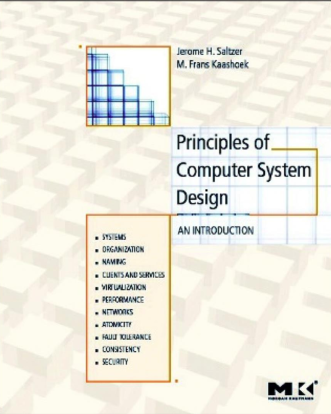
\includegraphics[scale=1.5]{S&K_P1.png}
            \caption*{\centering{Principles of Computer Systems Design Part:I \\by Saltzer and Kaashoek}}
        \end{minipage}
    \end{figure}
    \item Learning the bash Shell
    \item Managing Projects with GNU Make
    \begin{figure}[H]
        \centering
        \begin{minipage}{0.48\textwidth}
            \centering
            
\includegraphics[scale=1.5]{Learning_the_bash.png}
            \caption*{\centering{Learning the Bash Shell \\by Newham \& Rosenblatt}}
        \end{minipage} \hfill
        \begin{minipage}{0.48\textwidth}
            \centering
            
\includegraphics[scale=1.5]{managing_projs_with_GNU_make.png}
            \caption*{\centering{Managing Projects with GNU Make\\ by Mecklenburg}}
        \end{minipage}
    \end{figure}
    
\end{enumerate}

\begin{center}
	\rule{450pt}{1pt} 
\end{center}

\subsection*{What is this Doc?}
\addcontentsline{toc}{subsection}{What is this Doc?} 

This doc will contain my "notes" from each lecture of the class CSE130 at UCSC, taught by Prof. Kerry Veenstra. I shall divide this doc based on each lecture, and under each lecture write the important concepts/ideas talked about that day and other stuff I think is interesting. I may add some additional information/explanations from other sources. This is meant to be a comprehensive study doc for this class.
\begin{center}
	\rule{450pt}{3pt} 
\end{center}
\newpage

\section*{Lecture 1:}
\addcontentsline{toc}{section}{Lecture 1} 


\subsection*{What does class cover?}
\addcontentsline{toc}{subsection}{What does class cover?} 

\begin{enumerate}
    \item \textbf{Some Basic System Design Concepts} (Covered in S\&K)
    \item \textbf{Writing Multitasking C Programs} 
\end{enumerate}

\subsection*{Topics Covered}
\addcontentsline{toc}{subsection}{Topics Covered} 


\begin{minipage}[t]{0.45\textwidth} % First column
    \begin{itemize}
        \item Unix File I/O
        \item "Fundamental Abstractions"
        \item Client-Server Model
        \item Virtualization (also how the kernel works to virtualize: fork, exec, wait)
        \item Synchronization
        \item performance
        \item Security
    \end{itemize}
\end{minipage}%
\hfill
\begin{minipage}[t]{0.45\textwidth} % Second column
    \begin{itemize}
        \item Using pthreads
        \begin{itemize}
            \item[$\rightarrow$] Creating/joining threads
            \item[$\rightarrow$] Mutexes
            \item[$\rightarrow$] Condition Variables
            \item[$\rightarrow$] Synchronization
            \item[$\rightarrow$] Locks
        \end{itemize}
    \end{itemize}
\end{minipage}

\

\

Some of the above topics are from S\&K, the others are covered to enable you to do the assignments.

\subsection*{Programming Assignments}
\addcontentsline{toc}{subsection}{Programming Assignments}

\begin{itemize}
    \item \textbf{asgn0} --- Practice submitting assignments
    \item \textbf{asgn1} --- Command-line Memory
    \item \textbf{asgn2} --- HTTP Server
    \item \textbf{asgn3} --- Multi-Producer/Multi-Consumer Shared-Memory Queue (with updated features)
    \item \textbf{asgn4} --- Multi-Threaded HTTP Server (with updated features)
    \item \textbf{asgn5} --- Caching
\end{itemize}

\subsection*{Grade Breakdown:}
\addcontentsline{toc}{subsection}{Grade Breakdown:}

\begin{itemize}
    \item Five In-person Quizzes (\textbf{30\%})
    \item Six Programming Assignments (\textbf{50\%})
    \item Final Exam (\textbf{20\%})
\end{itemize}
 
\subsection*{On Using ChatGPT in this class}
\addcontentsline{toc}{subsection}{On Using ChatGPT in this class}

\begin{itemize}
    \item Prof. Veenstra asked his friends/peers in industry what it is that they do, when it comes to using generative AI. He got 2 kinds of answers.
    \item The first answer was that the company doesn't want them putting confidential information into prompts, but they have internal systems that are trained outside of OpenAI etc. So they can use an internal generative AI system that wont leak company secrets out into other peoples prompts.
    \item The other answer was, 
    \begin{enumerate}
        \item Read \& understand assignment PDF.
        \item Understand the \textbf{parts} of the assignment.
        \item Ask ChatGPT to show \textbf{3 different ways} to do one of the parts.
        \item Read, understand, and write that part based on your understanding.
        \item If needed, repeat this process for the other parts of the assignment.
    \end{enumerate}
    \item Your default role in our society is to be a consumer. A consumer of goods, services, entertainment(where you are the product). But you can decide to perform a different role than the one given to you by default, you can choose to be a Creator, Inventor or Researcher.
    \item If you give ChatGPT your Assignment PDF and then try to fix the mistakes it made in the generated code you have essentially \textbf{inverted the relationship}, you are giving ChatGPT the \textbf{creative} role and you are working as its \textbf{assistant}. You, as a human being, should perform the creative role.
\end{itemize}

\begin{center}
	\rule{450pt}{1pt} 
\end{center}
\newpage

\section*{Lecture 2}
\addcontentsline{toc}{section}{Lecture 2} 

\textbf{\large Required Pre-Lecture Reading: } S\&K Chapter 1: Systems.\\
\noindent For this lecture, my notes follow the general structure in the lecture slides, but at instances I elaborate a little more by taking material from the pre-lecture reading.

\

\noindent Modern computer systems are large \& \textbf{complex}.
\\
 This lecture covers:
\begin{itemize}
    \item What problems arise in designing \textbf{complex} computer systems?
    \item How can we manage the \textbf{complexity} and the resulting problems?
\end{itemize}

\subsection*{What is a System:}
\addcontentsline{toc}{subsection}{What is a System}
\begin{itemize}
    \item "A set of \textbf{interconnected components} that has an expected behavior observed at the \textbf{interface} with its \textbf{environment}."
    \item The underlying idea of the concept of system is to divide all the things in the
    world into two groups: those under discussion and those not under discussion.
\end{itemize}

\begin{figure}[H]
    \centering
    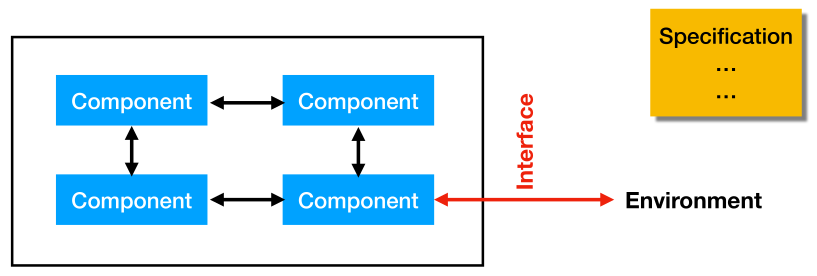
\includegraphics[scale=2.2]{System.png}
    \caption*\centering{System and Environment}
\end{figure}

\subsection*{Complexity}
\addcontentsline{toc}{subsection}{Complexity}
\begin{itemize}
    \item Four Issues of Complexity
    \item Signs of Complexity
    \item What are sources of System Complexity?
    \item What increases Complexity?
    \item How can we manage Complexity?
\end{itemize}

\subsection*{\underline{Four Issues of Complexity}}

\addcontentsline{toc}{subsection}{Four Issues of Complexity}
\begin{enumerate}
    \item \textbf{Emergent Properties}
    \begin{itemize}
        \item Emergent Properties are properties that are not evident in the individual components of a system but show up when combined.
        \item There can always be a argument about whether or not careful enough prior analysis of the components might have allowed prediction of the emergent behavior. It is wise to avoid this argument and instead focus on the fact that, some things turn up only when a system is built.
        \item [] Some Examples:
        \begin{itemize}
            \item The behavior of a committee(e.g. jury) can develop a way of thinking that could not have been predicted from knowledge about the individuals.
            \item The Tacoma Narrows Bridge, due to a combination of closed trusses and wind vortexes gave rise to torsional oscillation(emergent property) which led to the bridge collapsing.
            \item The Millennium Bridge became wobbly because of the way pedestrians synchronize their footsteps when the bridge sways, causing it to sway even more.
        \end{itemize} 
    \end{itemize}
    \item \textbf{Propagation of effects}
    \begin{itemize}
        \item Problems in one component of a system affects other components. The relationship between the components isn't always obvious.
        \item "There are no small changes in a large system."
        \item [] Some Examples:
        \begin{itemize}
            \item A tree falling on a power line in Oregon leads to the lights going out in New Mexico, $1000$ miles away.
            \item Santa Cruz 911 failure of 2009. Vandals cut fiber-optic communication cables in Santa Clara county, this causes Santa Cruz 911 to fail.
            \item Northeast Blackout of 1965, on a very cold winter evening, there was high power demand which caused a mis-programmed protection relay to trip under acceptable loads which caused a cascade of line overloads.
        \end{itemize}

    \end{itemize}
    \item \textbf{Incommensurate(not proportional) Scaling}
    \begin{itemize}
        \item Not all parts of a system scale at the same rate.
        \item The mathematical description of this problem is that different parts of the system exhibit different orders of growth.
        \item[] Some Examples:
        \begin{itemize}
            \item A mouse scaled up to the size of an elephant will collapse under its own weight, because the weight grows with volume(which is proportional to cube of linear size) while bone strength is proportional to its cross-sectional area(which is proportional to square of linear size).
        \end{itemize}
    \end{itemize}

    \item \textbf{Tradeoffs}
    \begin{itemize}
        \item What will I sacrifice for more of something else?
        \item The general model of a trade-off begins with the observation that there is a limited amount of some form of goodness in the universe, \& the design challenge is first to maximize that goodness, second to avoid wasting it, \& third to allocate it to the places where it will help the most.
        \item[] Some Examples:
        \begin{itemize}
            \item Bigger smartphones have bigger displays(positive) but use more battery(negative) and don't fit in pocket(negative).
            \item In context of integrated circuits, smaller transistor dimensions causes it to be faster(positive), but leads to more power consumption(negative) and more heating(negative).
            \item With Binary Classification, we often use a \textit{proxy} to classify or detect something. As a consequence of using a proxy there will be classification errors, "where should the threshold be?". When using a Smoke detector for detecting fire, we use smoke as the proxy and make a detector for that, but we don't wan't alarm to go off for normal cooking but also don't want ti to miss a real fire. Similar argument for a Spam email filter.
        \end{itemize}
    \end{itemize}
\end{enumerate}

\subsection*{\underline{Signs of Complexity}}
\addcontentsline{toc}{subsection}{Signs of Complexity}

\begin{itemize}
    \item Complex means “difficult to understand”. Lack of systematic understanding is the underlying feature of complexity. 
    \item Complexity is both a subjective and a relative concept, there is no unified measure of complexity. We instead look for signs/symptoms of it and if enough appear, argue that complexity is present.
\end{itemize}

\begin{enumerate}
    \item \textbf{Large number of components}
    \item \textbf{Large number of interconnections}
    \begin{itemize}
        \item Even a few components may be interconnected in an unmanageably large number of ways.
        \item[] Some Examples:
        \begin{itemize}
            \item Sun and the
            known planets comprise only a few components, but every one has gravitational attraction for every other, which leads to a set of equations that are unsolvable.
            \item (counterexample) Certain Crystals are not Complex, even though they have many components and interconnections because they have regular/symmetric structure.
        \end{itemize}
    \end{itemize}
    \item \textbf{Lots of irregularities(little differences)}
    \begin{itemize}
        \item By themselves, a large number of components and interconnections may still represent a simple system, if the components are repetitive and the interconnections are regular. However, a lack of regularity, as shown by the number of exceptions or by non-repetitive interconnection arrangements, strongly suggests complexity.
        \item Exceptions complicate
        understanding.
    \end{itemize}
    \item \textbf{Long description}
    \begin{itemize}
        \item “Kolmogorov complexity” of a computational object is the length of its shortest specification. The longer the Kolmogorov complexity the more complex the system.
        \item On the other hand, lack of a methodical description may also indicate that the system is complex.
    \end{itemize}
    \item \textbf{Large team of designers, implementers, or maintainers}
    \begin{itemize}
        \item Several people are required to understand, construct, or maintain the system. A fundamental issue in any system is whether or not it is simple enough for a single person to understand all of it. If not, it is a complex system.
        \item This is the weakest indicator of complexity.
    \end{itemize}
\end{enumerate}

One objection to conceiving complexity as being based on the five signs is that all systems are indefinitely, perhaps infinitely, complex because the deeper one digs the more signs of complexity turn up. Thus, even the simplest digital computer is made of gates, which are made with transistors, which are made of silicon, which
is composed of protons, neutrons, and electrons, which are composed of quarks, which some physicists suggest are describable as vibrating strings, and so on. We shall address this objection in a moment by \textbf{limiting the depth of digging}, a technique
known as \textbf{abstraction}. The complexity that we are interested in and worried about is the complexity that remains despite the use of abstraction.


\subsection*{\underline{Sources of System Complexity}}
\addcontentsline{toc}{subsection}{Sources of System Complexity}

\begin{enumerate}
    \item \textbf{Interaction of Requirements}
    \begin{itemize}
        \item A primary source of complexity is just the list of requirements for a system.
        \item Each requirement, viewed by itself may even appear to add only easily tolerable complexity to an existing list of requirements.
        \item The problem is that the accumulation of many requirements adds not only their individual complexities but also complexities from their interactions.
        \begin{tcolorbox} [title= Design Principle:, colback=black!10!white]
            \centering{\textbf{Principle of Escalating Complexity}}\\
            Adding a requirement increases complexity out of proportion.
        \end{tcolorbox}

        \item Interaction complexity arises from pressure for generality and exceptions that add complications, it's made worse by change in individual requirements over time.
        \item Meeting many requirements with a single design is expressed as a need for generality. There's a tension between exceptions and generality.
        \begin{tcolorbox} [title= Design Principle:, colback=black!10!white]
            \centering{\textbf{Avoid Excessive Generality}}\\
            If it's good for everything, it's good for nothing.
        \end{tcolorbox}
    \end{itemize}

    \item \textbf{Increasing efficiency, utilization, or other measure of "goodness"}
    \begin{itemize}
        \item The "low-hanging fruit" is easy to get, i.e., if there is an optimization that is obvious and simple to implement, it is already(or will soon be) done, but the subsequent optimizations will be harder and harder to make.
        \item Additional gains in efficiency require more complexity. As a general rule, the more one tries to increase utilization of a limited resource, the greater the complexity. 
        \begin{tcolorbox} [title= Design Principle:, colback=black!10!white]
            \centering{\textbf{The law of diminishing returns}}\\
            The more one improves some measure of goodness, the more effort the next improvement will require.
        \end{tcolorbox}
    \end{itemize}

\end{enumerate}


\subsection*{\underline{What Increases Complexity?}}
\addcontentsline{toc}{subsection}{What Increases Complexity?}
(Essentially repeating each of the design principles mentioned.)
\begin{enumerate}
    \item \textbf{Principle of Escalating Complexity}
    \begin{itemize}
        \item Adding a requirement increases complexity out of proportion.
        \item[] Some Examples:
        \begin{itemize}
            \item If you want to make your microprocessor go faster and you have already done all the circuit design tricks that you can think of, then the only way to increase speed is to do things like branch prediction, super-scalar, register renaming etc. all these make the system even more complicated.
        \end{itemize}
    \end{itemize}
    \item \textbf{Principle of Excessive Generality}
    \begin{itemize}
        \item If it's good for everything, it's good for nothing.
        \item[] Some Examples:
        \begin{itemize}
            \item Amphicar(car+boat), ended up being a subpar boat and a subpar car. Same problem with "flying cars".
        \end{itemize}
    \end{itemize}
    \item \textbf{Law of diminishing returns}
    \begin{itemize}
        \item The more one measure of goodness is improved, the harder it gets to make the next improvement.
        \item[] Some Examples:
        \begin{itemize}
            \item If you want a faster computer system, you add cache memory, if you want it to be faster still, you can go onto adding a bucket list of every more complicated optimizations like branch prediction, super-scalar etc, but the return on investment(in terms of speed) keeps getting lesser and lesser.
        \end{itemize}
    \end{itemize}
\end{enumerate}

\subsection*{\underline{Managing Complexity}}
\addcontentsline{toc}{subsection}{Managing Complexity}

\begin{enumerate}
    \item \textbf{Modularity}
    \begin{itemize}
        \item Modularity is the technique of breaking things into smaller pieces(aka divide-and-conquer), it's essentially analyzing or designing the system as a collection of interacting subsystems, called modules.
        \item The power of this technique lies in being able to consider interactions among the components within a module without simultaneously thinking about the components that are inside other modules.
        \item Modularity allows development of a smaller unit, that reduces the number of components and interactions, that reduces complexity and reduces the number of bugs.
        \item Modularity makes it easy to replace an inferior module with an improved one, thus allowing incremental improvement of a system without completely rebuilding it. Modularity thus helps control the complexity caused by change.
        \begin{tcolorbox} [title= Design Principle:, colback=black!10!white]
            \centering{\textbf{The unyielding foundations rule}}\\
            It is easier to change a module than to change the modularity.
        \end{tcolorbox}
        \item[] Some Examples:
        \begin{itemize}
            \item Consider debugging a large program with \lstinline|N| statements. Assume number of bugs in the program is proportional to its size and the bugs are randomly distributed.
            $$ \text{BugCount}\sim \text{\lstinline|N|}$$
            Assume also that the time taken to find a bug in a program is roughly proportional to the size of the program.
            \begin{eqnarray*}
                \text{DebugTime}&\sim&\text{\lstinline|N|}\times\text{BugCount}\\
                &\sim& \text{\lstinline|N|}^2
            \end{eqnarray*}
            Suppose the program is divided into \lstinline|K| modules, each roughly equal size, so now the modules contain \lstinline|N/K| statements.\\
            The time required to debug any one module is thus reduced in two ways: the smaller module can be debugged faster, \& since there are fewer bugs in smaller programs, any one module will not be needed to be debugged as many times. Thus the time required to debug the system of \lstinline|K| modules becomes,
            \begin{eqnarray*}
                \text{DebugTime}&\sim&\left(\frac{\text{\lstinline|N|}}{\text{\lstinline|K|}}\right)^2\times \text{\lstinline|K|}\\
                &\sim& \frac{\text{\lstinline|N|}^2}{\text{\lstinline|K|}}
            \end{eqnarray*}
            Therefore we can see that modularization into \lstinline|K| components reduces debugging time by a factor of \lstinline|K|.
        \end{itemize}
    \end{itemize}
 
    \item \textbf{Abstraction}
    \begin{itemize}
        \item When using modularity to subdivide a complex system, it should be noted that the best divisions usually follow natural or effective boundaries. They are characterized by fewer interactions among modules \& cause less propagation of effects from one module to another.
        \item More generally, they are characterized by the ability of any module to treat all the others entirely on the basis of their external specification, without need for knowledge about what goes on inside.
        \item This additional requirement on modularity is called \textbf{abstraction}. Abstraction is separation of interface from internals, or specification from implementations. Essentially treating the individual components of a system as a \textbf{black box}. The black box has inputs \& outputs \& behaviors. You are Supposed to trust that the black box will do what it promises. 
        \item Abstraction nearly always accompanies modularity. The term \textit{functional modularity} is used to mean modularity with abstraction
        \begin{tcolorbox} [title= Design Principle:, colback=black!10!white]
        \centering{\textbf{The robustness principle}}\\
            Be tolerant of inputs and strict on outputs.
        \end{tcolorbox}
        \item The effect of the robustness principle is to suppress, rather than propagate or even amplify, noise, or errors that show up in the interfaces between modules.
        \item[] Some Examples:
        \begin{itemize}
            \item Programs are designed to hide details of their representation of complex data structures and details of which other programs they call. Users expect an easy-to-use user interface that abstracts incredibly complex underpinnings pf memory, processor, communication, and display management.
            \item A market economy is characterized by modularity. Rather than having a self-supporting farm family that
            does everything for itself, a market economy has coopers, tinkers, blacksmiths, stables, dressmakers, and so on, each being more productive in a modular specialty, all selling things to one another using a universal interface—money.
        \end{itemize}
    \end{itemize}

    \item \textbf{Layering}
    \begin{itemize}
        \item Systems that are designed using good abstractions tend to minimize the number of interconnections among their component modules. 
        \item One powerful way to reduce module interconnections is to employ a particular method of module organization known as \textbf{layering}. In designing with layers, one builds on a set of mechanisms that is already complete(a lower layer) and uses them to create a different complete set of mechanisms(an upper layer).
        \item A layer may itself be implemented as several modules, but as a general rule, a module of a given layer interacts only with its peers in the same layer and with the modules of the next higher and next lower layers.
        
        \begin{figure}[H]
            \centering
            \begin{minipage}{0.48\textwidth}
                \centering
                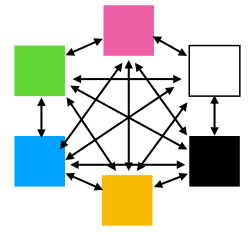
\includegraphics[scale=2]{No_Layering.png}
                \caption*{\centering{No Layering}}
            \end{minipage} \hfill
            \begin{minipage}{0.48\textwidth}
                \centering
                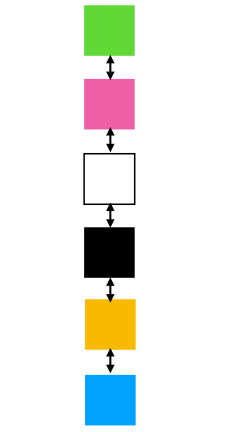
\includegraphics[scale=2]{Layering.png}
                \caption*{\centering{Layering}}
            \end{minipage}
        \end{figure}
        \begin{tcolorbox}[
            title=Fundamental theorem of software engineering (David Wheeler):, 
            colback=gray!5!white,         % Light gray background
            colframe=black!80,           % Dark gray border
            colbacktitle=gray!20!white,  % Medium gray title background
            coltitle=black,              % Black text for the title
            fonttitle=\bfseries,         % Bold title font
            sharp corners                % Ensures rectangular corners
        ]
            "Any problem in computer science can be solved with another layer of indirection, \textcolor{red}{except for the problem of too many layers of indirection}."
        \end{tcolorbox}
        \item[] Some Examples:
        \begin{itemize}
            \item Nearly every computer system comprises several layers. The lowest layer consists of transistors, gates and memory cells, upon which is built a layer consisting of a processor and memory. On top of this layer is built an OS layer, which acts as an augmentation of the processor and memory layer. Finally an application program executes on this augmented processor and memory layer.
            \begin{figure}[H]
                \centering
                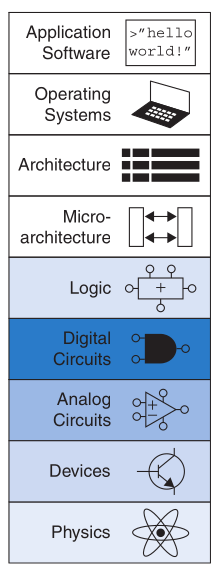
\includegraphics[scale=1.8]{levels_of_abstraction.png}
                \caption*\centering{Levels of abstraction for an electronic computing system}
            \end{figure}
        \end{itemize}
    \end{itemize}

    \item \textbf{Hierarchy}
    \begin{itemize}
        \item The final major technique for coping with complexity also reduces interconnections among modules. 
        \item Start with a small group of modules, and assemble them into a stable, self-contained subsystem that has a well-defined interface. Next assemble a small group of subsystems to produce a larger subsystem. This process continues until the final system has been constructed from a small number of relatively large subsystems.
        \item The result is a tree-like structure known as a \textbf{hierarchy}.
        \item Hierarchy constrains the interactions by permitting them only among the components of a subsystem. Hierarchy constrains a system of $N$ components, which in the worst case might exhibit $N\times(N-1)$ interactions, so that each component can interact only with members of its own subsystem, except for an interface component that also interacts with other members of the subsystem at the next higher/lower level of hierarchy.
        \item Analogous to the way that modularity reduces the effort of debugging, Hierarchy reduces the number of potential interactions among modules from square-law to linear.
        \begin{figure}[H]
            \centering
            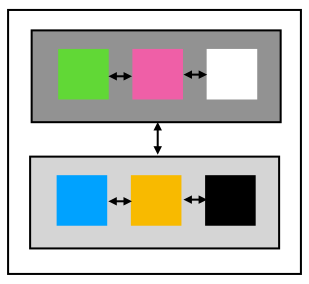
\includegraphics[scale=1.8]{hierarchy.png}
            \caption*\centering{System broken into subsystems broken into modules}
        \end{figure}
    \end{itemize}

    \item \textcolor{red}{\textbf{Naming (We don't cover this in CSE-130)}}
    FILL THIS UP SOME TIME
\end{enumerate}
 
\begin{center}
	\rule{450pt}{1pt} 
\end{center}
\newpage

\section*{Lecture 3}
\addcontentsline{toc}{section}{Lecture 3}

\begin{itemize}
    \item Prof. Veenstra worked through Prof. Quinn's Practicum for setting up your system for CSE 130, this included,
    \begin{itemize}
        \item Installing \& setting up Multipass VM.
        \item Setting up the respective repositories(there are 2, named $<$your cruz-id$>$ and resources).
        \item Setting up and using the auto-grader.
        \item Using the resources repo for loading local test cases.
    \end{itemize}
    \item Had Quiz 1---On the material from Lecture 2(Complexity).
\end{itemize}
\begin{center}
	\rule{450pt}{1pt} 
\end{center}
\newpage

\section*{Lecture 4}
\addcontentsline{toc}{section}{Lecture 4}

\subsection*{Review of C Strings/Variables}
\addcontentsline{toc}{subsection}{Review of C Strings/Variables}

\subsection*{UNIX File I/O}
\addcontentsline{toc}{subsection}{UNIX File I/O}





\begin{center}
	\rule{450pt}{1pt} 
\end{center}
\newpage

\section*{Lecture 5}
\addcontentsline{toc}{section}{Lecture 5}





\begin{center}
	\rule{450pt}{1pt} 
\end{center}
\newpage

\section*{Lecture 6}
\addcontentsline{toc}{section}{Lecture 6}





\begin{center}
	\rule{450pt}{1pt} 
\end{center}
\newpage

\section*{Lecture 20}
\addcontentsline{toc}{section}{Lecture 20}

\subsection*{Refresher: SI Prefixes}

\begin{table}[h]
    \centering
    \begin{tabular}{|c|c|c|}
        \hline
        Prefix & Power(base 2) & Power(base 10) \\
        \hline
        Kilo(k) & $2^{10}$ & $10^3$\\
        Mega(M) & $2^{20}$ & $10^6$\\
        Giga(G) & $2^{30}$ & $10^9$\\
        \hline
        Milli(m) & $2^{-10}$ & $10^{-3}$\\
        Micro($\mu$) & $2^{-20}$ & $10^{-6}$\\
        Nano(n) & $2^{-30}$ & $10^{-9}$\\
        \hline
    \end{tabular}
    \caption*{Commit these to memory}
    \label{tab:example}
\end{table}

\subsection*{Computer Systems performance}

\begin{itemize}
    \item We want computers to perform "Better":
    \begin{itemize}
        \item Increase Throughput.
        \item Decrease Latency.
        \item Get more things done per unit of energy.
    \end{itemize}
\end{itemize}

\subsection*{How is performance measured?}

\subsubsection*{Capacity Metrics:}
\begin{itemize}
    \item \underline{\textbf{Capacity:}} Amount of a resource thats available.
    \begin{itemize}
        \item Eg: This machine has a \textbf{8Gb} RAM.
    \end{itemize}
    \item \underline{\textbf{Utilization:}} Percentage of Capacity being used for a given workload.
    \item \underline{\textbf{Overhead:}} Resource that is "wasted".
    \begin{itemize}
        \item Eg: In a layered system, layers below are Overhead.
    \end{itemize}
    \item \underline{\textbf{Useful Work:}} Resource spent on actual work for a given workload.
    \begin{itemize}
        \item In a layered system, layers above perform useful work.
    \end{itemize}
\end{itemize}

\subsubsection*{Time-based metrics:}
\begin{itemize}
    \item \underline{\textbf{Latency:}} Elapsed time for a \textbf{single} action.
    \item \underline{\textbf{Throughput:}} \textbf{Rate} of actions per unit time(also called "bandwidth"). 
\end{itemize}

\subsection*{System Latency and Throughput}
\begin{itemize}
    \item Latency and Throughput are 2 different things but there can be a relationship between them.
    \item If you have a single module(1 stage), the time to get the data from the input of the module to the output(the latency), assuming its not pipelined is related to the Throughput as: 
    $$\text{Latency}=\frac{1}{\text{Throughput}}$$
    \begin{figure}[H]
        \centering
        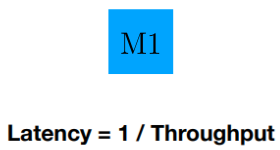
\includegraphics[scale=2.2]{Latency_Throughput.png}
        \caption*\centering{Blue Box represents a single module}
    \end{figure}
    In this case the module cannot process more than one thing at a time.
    \item Instead if we did pipelining and we have some concurrency, then the total latency and Throughput of the entire pipelined system is:
    $$\text{Total Latency}=\text{sum(module Latencies)}$$ 
    $$\text{Total Throughput}=\text{min(module Throughputs)}$$
    \begin{figure}[H]
        \centering
        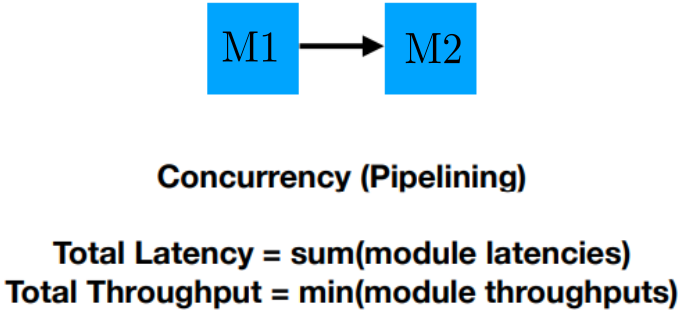
\includegraphics[scale=1.5]{pipelined.png}
        \caption*\centering{Blue Box represents a single module}
    \end{figure}
    \item Another way to do concurrency is to have modules running parallelly. The two cases here are if all the modules are identical or if all the modules are different. In the second more general case the average latency of the entire system will be a weighted average of the Latencies of its component modules. In the second case the throughput depends on how the requests get distributed i.e. you need to know what fraction/percentage of the incoming data is going through one of the modules and what percentage is going through the other module.
    \begin{figure}[H]
        \centering
        \begin{minipage}{0.48\textwidth}
            \centering
            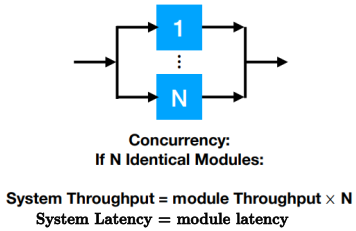
\includegraphics[scale=2.5]{parallel.png}
        \end{minipage} \hfill
        \begin{minipage}{0.48\textwidth}
            \centering
            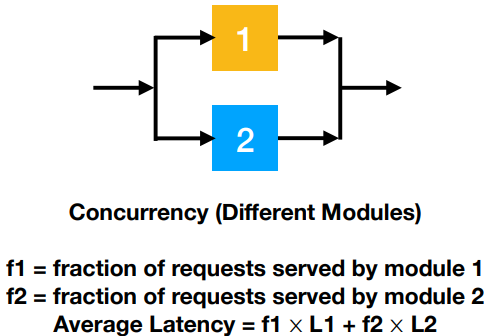
\includegraphics[scale=1.8]{diff_modules.png}
        \end{minipage}
    \end{figure}
    \item There can be a situation in which the the rates of the input \& output on either side of the module differ, then the minimum of the two throughputs is the fastest throughput the module can have.
    \begin{figure}[H]
        \centering
        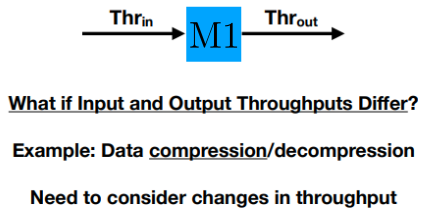
\includegraphics[scale=2]{diff_throughputs.png}
    \end{figure}
\end{itemize}

\subsection*{Techniques for Improving System performance:}
\begin{enumerate}
    \item Pipelining
    \item Concurrency
    \item Fast Path
    \item Limitations
\end{enumerate}

\subsection*{1. Pipelining}
\begin{itemize}
    \item \underline{\textbf{Pipelining:}} Split operation into multiple individual stages.
    \begin{itemize}
        \item Each stage operates independently.
        \item Single request goes through multiple stages.
        \item Different requests may go through different stages.
    \end{itemize}
    \item Latency: The time for a single request to go through all stages.
    $$\text{latency}_{A+B}\ge \text{latency}_A + \text{latency}_B\footnote{$\ge$ because there can be overhead of the transition between the pipelined stages}$$
    \item Throughput: The net throughput of the system is limited by the throughput of the slowest stage.
    $$\text{throughput}_{A+B}\le(\text{throughput}_A+\text{throughput}_B)$$
    \item Pipelines increase throughput by keeping every stage of the system busy.
\end{itemize}

\subsection*{2. Concurrency}
\begin{itemize}
    \item Concurrency can \textbf{reduce latency}, by running independent parts of stages in parallel.
    \item Concurrency can \textbf{increase throughput}, because each stage works on a different request.
\end{itemize}

\subsection*{3. Fast Path}
\begin{itemize}
    \item Reducing latency is difficult: often limited by:
    \begin{itemize}
        \item Speed of light
        \item Algorithm run time
    \end{itemize}
    \item We can Leverage the non-uniformity: reduce latency for some requests, by creating a fast path.
    \item One very common approach to fast-pash is Caching.
    \item In caching we have a fast memory(which we call the fastpath) and we have the larger slow memory. The fast memory tends to be faster but only contains a subset of the data, the slow memory is large enough to contain all the data, if you can design your system in a way such that most of your data requests are serviced by the fast small memory, even though it only has a subset of all the data. Then it appears as if you have a large memory as fast as the faster small memory.
\end{itemize}



%----------------------------------
\newpage


\definecolor{lightblue}{RGB}{178,205,224}
\definecolor{darkblue}{RGB}{0,88,159}
\definecolor{blacklogic}{RGB}{0,0,0}
\begin{tcolorbox}[
    colback=lightblue,    % Background color of the box
    colframe=darkblue,    % Border color of the box
    coltitle=white,  % Color of the title text
    fonttitle=\bfseries,  % Bold title text
    title=Digital Circuits
]
This is a tcolorbox using the color palette inspired by your image.
\end{tcolorbox}




\begin{center}
	\rule{450pt}{4pt} 
\end{center}
\newpage

\section*{\centering\underline{Complexity Cheat Sheet}}
\addcontentsline{toc}{section}{Complexity Cheat Sheet}


\subsection*{Complexity}
\begin{enumerate}
    \item Four Issues of Complexity
    \item Signs of Complexity
    \item What are Sources of System Complexity?
    \item What Increases Complexity?
    \item How Can We Manage Complexity?
\end{enumerate}
\begin{center}
	\rule{450pt}{1pt} 
\end{center}

\noindent\large{\textbf{1. Four Issues of Complexity}}
\begin{enumerate}
    \item Emergent Properties
    \item Propagation of effects
    \item Incommensurate Scaling
    \item Tradeoffs
\end{enumerate}

\

\noindent\large{\textbf{2. Signs of Complexity}}
\begin{itemize}
    \item Large number of components
    \item Large number of interconnections
    \item Lots of irregularities \ (little differences)
    \item Long description \ (high information content)
    \item Large team of designers \ ("weakest" Symptom)
\end{itemize}

\

\noindent\large{\textbf{3. What are Sources of System Complexity?}}
\begin{itemize}
    \item Interactions of requirements
    \item Increasing efficiency, utilization, or other measure of "goodness"
\end{itemize}

\

\noindent\large{\textbf{4. What Increases Complexity?}}
\begin{itemize}
    \item Principle of escalating complexity
    \item Principle of excessive generality
    \item Law of diminishing returns
\end{itemize}

\

\noindent\large{\textbf{5. How Can We Manage Complexity?}}
\begin{itemize}
    \item Modularity
    \item Abstraction
    \item Layering
    \item Hierarchy
    \item \textcolor{red}{Naming}
\end{itemize}
\newpage


\end{document}
